\section{Grundlagen}\label{sec:Grundlagen}

Wie schon zu Beginn erwähnt, sollen in diesem Abschnitt der Ausarbeitung die Grundlagen der von uns verwendeten Technologien und Konzepte angesprochen und näher erläutert werden. Zu Beginn werden die eingesetzten Werkzeuge und die Konfiguration der Entwicklungsumgebung besprochen. Anschließend sollen grundlegende Kenntnisse der Webentwicklung mit \ac{JSF} und PostgreSQL vermittelt werden.

\subsection{Eclipse und Entwicklungsunterstützung}
Umfangreiche Softwareprojekte lassen sich durch die Verwendung einer \gls{Integrated Development Environment} (IDE) wie \gls{Eclipse} oder \gls{NetBeans} besser bearbeiten. 
Eclipse wurde ursprünglich von IBM entwickelt und im Jahr 2001 quelloffen veröffentlicht. Im Jahre 2004 übernahm die \gls{Eclipse-Foundation} die Weiterentwicklung des Projekts und ist heute neben der \gls{Apache Software Foundation} eines der größten Open-Source-Communities im Bereich der JAVA-Softwareentwicklung.
Seit dem Jahr 2006 wurden verschiedene Versionen und Unter-Projekte von Eclipse auf einen gemeinsamen und aktuellen Stand gebracht.
Nach vielen Jahren der Entwicklung und stetigen Verbesserungen ist Eclipse heutzutage eines der beliebtesten IDEs im Bereich der Anwendungsentwicklung.
Heute ist Eclipse weit davon entfernt, eine IDE nur für JAVA zu sein. Diverse Erweiterungen machten es zu dem Entwicklungstool für Software jeglicher Art und beinahe jeglicher Programmiersprache schlechthin.

Für die Entwicklung der Projektarbeit selbst, wurde Eclipse Version 4.2 (Juno) verwendet.
Außer den Basisfunktionen stehen Entwicklern viele Möglichkeiten offen, diverse Plug-ins und Tools in Eclipse zu integrieren, die die Arbeit erleichtern.

Die für dieses Projekt verwendeten Softwareunterstützungen waren:
\begin{itemize}
	\item \gls{Apache Maven}
	\item Eclipse \ac{WTP}
	\item JBoss-Tools
	\item Git-Repository
\end{itemize}
  
Juno selbst stellt standardmäsig bereits über die Enterprise Edition, das Projekt WTP, eine Unterstützung für die Entwicklung von JSF bereit. 
Eine weiteres Tool, die \gls{JBoss}-Tools, welche auch eine Erweiterung der Entwicklungsunterstützung im aktuellen Projekt darstellen, werden im übernächsten Unterabschnitt noch genauer erklärt.

Zur Automatisierung einzelner Schritte in der Softwareentwicklung wurde das Build- und Management-Tool Apache Maven zur Umsetzung verwendet. 

Desweiteren kam die freie Software zur Versionsverwaltung \gls{Git} zum Einsatz. Software dieser Art bietet sich vorallem bei kollaborativen Projekten, also Projekten mit mehreren Entwicklern, an. 
Aber auch der Vorteil der Versionskontrolle bei kleinen 'Ein-Mann-Projekten' soll besser nicht unterschätzt werden.

Da es sich hier um selbstständige Tools handelt, die nicht zwingend in einer IDE integriert sein müssen, werden diese jeweils in einem eigenen Unterabschnitt genauer erklärt.
Im Folgenden soll zuerst auf Maven eingegangen werden.

\subsection{Apache Maven}

Der sinnvollste Weg, ein \ac{JSF} Projekt zu verwalten, ist Apache Maven.
Das Tool wird von der \gls{Apache Software Foundation} entwickelt und dient zur Verwaltung von Softwareprojekten überwiegend im JAVA Umfeld. 

Für die Entwicklung und Integration von Maven in Eclipse bietet sich die Installation des Plugins \texttt{m2e} bzw. \texttt{m2eclipse} an. Die Integration und Verwendung von Maven in Eclipse ist unter \cite{EclM2E} näher beschrieben. 

Bei Maven steht vorallem die Integration der Webapp sowie die Bibliotheks- und Versionsverwaltung im Vordergrund. Die genaue Funktionsweise wird im späteren Verlauf noch erklärt. 
Das erstellte \gls{Apache Maven}-Projekt kann somit in Eclipse importiert und dort bearbeitet werden oder wird schon zu Beginn in Eclipse angelegt. 
Eine Integration von \gls{Apache Tomcat} in Eclipse bietet dann die Möglichkeit, die Webapp ohne umständliches Erstellen und Installieren auf dem \gls{Servlet-Container} zu verwenden.

% Maven Workflow
\begin{wrapfigure}[12]{r}{12cm}
\centering\begin{tikzpicture}[decoration=penciline, decorate]
  \node at (1,4) {Projekt Workspace};
  \node at (8,4) {Maven Repository};

  % Repo
  \draw[dashed, decorate,ultra thick] (0,-1) -- (0,3) -- (3,3) -- (3,-1) -- (0,-1);
  \draw[draw=black, fill=yellow!30!, opacity=0.4, decorate,thick] (1,1) -- (1,2.8) -- (2.8,2.8) -- (2.8,1) -- (1,1);
  \node[decorate] at (1.9, 2.5) {$POM$};
  \node[decorate] at (1, 0) {$/lib/$};

  % Pfeil
  \draw[->, color=black, out=50, in=190, thick] (2,2) to (8,2.5);
  \draw[->, color=black, out=20, in=170, thick] (2.8,0) to (8,1.5);

  % Libs
  \node[decorate, circle, fill, red, inner sep=4pt] at (2.3,-0.2) {};
  \node[decorate, circle, fill, red!20!, inner sep=4pt] at (2.1,0.2) {};
  \node[decorate, circle, fill, red!50!, inner sep=4pt] at (2,-0.5) {};
  \node[decorate, circle, fill, blue!60!, inner sep=4pt] at (1.8,-0.2) {};

  % Pfeil
  \draw[decorate, <-, color=black!50!white, out=270, in=180, thick] (1,-0.2) to (2,-1.6);
  \node[decorate] at (2,-1.8) {\textit{\small{...internes lib-Verzeichnis}}};

  % Maven Repo
  \draw[very thick] (8,2.5) ellipse (60pt and 20pt);
  \draw[very thick] (8,0) ellipse (60pt and 20pt);
  \draw[decorate, very thick] (6,0) -- (6,2.5);
  \draw[decorate, very thick] (10,0) -- (10,2.5);
\end{tikzpicture}
\caption[\textbf{Maven Verwaltung}]{Skizze der Maven Verwaltung}
\label{fig:Maven_Verwaltung}
\end{wrapfigure}

In \prettyref{fig:Maven_Verwaltung} wird die Verwaltung mit Hilfe von Maven dargestellt.

Ein grundlegendes Konzept von Maven lautet: 'convention over configuration' (Konvention vor Konfiguration).
Konkret bedeutet dies, dass sich Maven standardmäßig immer so verhält, wie es für die meisten Projekte sinnvoll ist und nur bei Abweichung von Normen konfiguriert werden soll.
Zu diesem Konzept gehört auch die Verzeichnisstruktur, die standardmäßig verwendet wird, bei Bedarf aber angepasst werden kann.

Der Aufbau einer Verzeichnisstruktur für Webandwendungen ist folgendermaßen aufgebaut:

Maven bildet die Quellen im Verzeichnis \texttt{src} und die lauffähige Version des Programms als \texttt{*.war} im Verzeichnis \texttt{target} ab. Dies beschreibt den Fall einer Standarkonfiguration für \gls{Apache Tomcat}-Webapplikationen. \gls{Apache Maven}-Projekte können aber auch anhand von \glspl{Archetype} erstellt werden. Dieses Projekt basiert auf einem 'Custom Project' welches JSF-myFaces Core 2.0 nutzt.

% Verzeichnisstruktur
\tikzstyle{every node}=[draw=black,thick,anchor=west]
\tikzstyle{selected}=[draw=black,fill=red!30]
\tikzstyle{optional}=[dashed,fill=green!40]
\tikzstyle{head}=[draw=black,fill=blue!30]
\tikzstyle{dots}=[draw=black,fill=yellow!30]
\tikzstyle{dirs}=[draw=black,fill=green!30]

\begin{wrapfigure}[21]{l}{10cm}
\centering
\begin{tikzpicture}[
  grow via three points={one child at (0.5,-0.7) and
  two children at (0.5,-0.7) and (0.5,-1.4)},
  edge from parent path={(\tikzparentnode.south) |- (\tikzchildnode.west)}]

    \node [head] {kuwasys20}
    child { node {$<$ECLIPSE RESSOURCES$>$}}
    child { node [selected] {pom.xml}}
    child { node [selected] {src}
      child { node {main}
    child { node {java}
      child { node [optional] {$<$JAVA Code$>$}}
    }
    child [missing] {}
    child { node {webapp}
      child { node [optional] {$<$FACELETS$>$}}
    }
      }
      child [missing] {}
      child [missing] {}
      child [missing] {}
      child { node {admin}}
      child { node {resources}
    child { node [dots] {...}}
      }
      child [missing] {}
      child { node [optional] {WEB-INF}
    child { node [dots] {...}}
      }
      child [missing] {}
    }
    child [missing] {}
    child [missing] {}
    child [missing] {}
    child [missing] {}
    child [missing] {}
    child [missing] {}
    child [missing] {}
    child [missing] {}
    child [missing] {}
    child [missing] {}
    child { node [selected] {target}
      child { node {m2e-wtp}
    child { node {web-resources}
      child { node [optional] {META-INF}
        child { node [dots] {...}}
      }
    }
      }
};
\end{tikzpicture}
\caption[\textbf{Maven Projekt Verzeichnisstruktur}]{Maven Projekt Verzeichnisstruktur}
\label{fig:Maven_Verzeichnis}
\end{wrapfigure}

Das Herzstück eines Maven-Projekts bildet das \ac{POM}, welches durch die Datei \texttt{pom.xml} repräsentiert wird. Ein Ausschnitt ist in \prettyref{lstmin:pom.xml} zu sehen.
Darunter finden sich unter anderem Informationen über die Art des Projekts, Angaben zur Art des Erstellvorgangs und Abhängigkeiten, wie z.B. der JSF-myFaces Core-\gls{API}, JSF-myFaces Tomahawk und PostgreSQL.

Mit dem Element \texttt{packaging} wird angegeben, dass das Projekt als WAR-Archiv gepackt werden soll.

Das Element \texttt{dependencies} enthält alle Softwareabhängigkeiten. Für jede Abhängigkeit wird ein \texttt{dependency}-Element angegeben. Es wird auch Artefakt genannt, welches mit \texttt{groupID}, \texttt{artifactID} und einer Versionsnummer beschrieben wird, welches in Kombination einzigartig ist.
Das Element \texttt{scope} gibt an, in welchem Classpath (Laufzeit, Kompilierzeit oder Ausführung von Tests) ein solches Artefakt verfügbar sein soll. Wichtige Werte für das Element sind:

\texttt{compile},

standardmäßig definiert. Es bedeutet, dass ein Artefakt in jedem Classpath vorhanden sein soll.

\texttt{provided},

Artefakte sind nur beim Kompilieren im Classpath enthalten und werden nicht in die fertige Anwendung integriert. Das ist dann sinnvoll, wenn Artefakte zum Kompilieren benötigt werden, aber beim Ausführen sich ohnehin im JDK befinden.

\texttt{runtime},

die Artefakte werden zum Ausführen und Testen benötigt, aber nicht zum Kompilieren. Sind sind in der fertigen Anwendung enthalten.

\texttt{test},

wenn Artefakte fürn Tests benötigt werden. Sie sind nicht in der fertigen Anwendung enthalten und außerdem nur beim Kompilieren und Ausführen von Tests verfügbar.
Alle hier aufgeführten \texttt{scopes} sind in \cite{MVNintrodep} zu finden. 

	%% Listing: git clone
	\lstinputlisting[label={lstmin:pom.xml},
	captionpos=b,
	belowcaptionskip=1pt,
	caption={Ausschnitt der \texttt{pom.xml}},
	frame=tlbr, 
	language=xml, 
	breaklines=true, 
	numbers=left,
	numberstyle=\tiny, 
	stepnumber=1, 
	numbersep=5pt, 
	basicstyle=\small\ttfamily,
	showstringspaces=true,
	keywordstyle=\bfseries\color{lila}, 
	backgroundcolor=\color{lightgrey}]{listings/pom.xml}

Beim Auflösen der Abhängigkeiten eines Projekts, bspw. während dem Kompiliervorgang, prüft Maven zunächst, an welcher Stelle sich benötigte Artefakte befinden. Zunächst wird das lokale Repository geprüft. Hierbei handelt es sich um ein Verzeichnis im lokalen Dateisystem.
Ist das nicht der Fall, versucht Maven sich die Artefakte über das Central Repository, einer durch Apache bereitgestellten Sammlung von Artefakten, herunterzuladen. 

\subsection{Verteilungs- und Versionskontrolle mit Git}

Wie bereits erwähnt, wurde das Projekt mit der Hilfe der Versionskontrolle Git realisiert. Git stellt, neben \gls{Subversion} (SVN) und \gls{Mercurial}, das beliebteste Werkzeug zur Verteilung von Daten mit Versionskontrolle dar.

\begin{wrapfigure}[8]{l}{7cm}
 \begin{center}
   
\includegraphics[scale=0.5]{img/git_logo.png}
 \end{center}
 \caption[\textbf{Git Logo}\protect\newline Quelle: \url{http://upload.wikimedia.org/wikipedia/commons/thumb/e/e0/Git-logo.svg/273px-Git-logo.svg.png}]{Git Logo}
 \label{fig:git_logo}
\end{wrapfigure}
\newpage

Entwickelt wurde Git ursprünglich für Aktualisierungen des Linux-Kernels. Es verbreitete sich jedoch schnell in Kreisen der Softwareentwicklung für Verteilung, Versionskontrolle und Backup.
Software dieser Art wird dazu verwendet, alle Dateien eines Projekts bei jedem Mitwirkenden aktuell und gleich zu halten. Ein weiterer Vorteil ist hierbei, dass auf jede beliebige Vorgängerversion zurückgegriffen werden kann. So kann bei schwerwiegenden Fehlern zu einer funktionstüchigen Version gesprungen werden. Der positive Nebeneffekt sind daher auch Backups des kompletten Projekts, die im sogenannten Git-Repository sind. 

Obwohl der Sinn und Zweck im Allgemeinen der gleiche ist, trifft man bei Git auf einige Unterschiede gegenüber traditionelleren Versionskontrollsystemen wie bspw. SVN, die kurz beschrieben werden sollen:

Die Verteilung der Daten wird nicht wie bei SVN über eine zentrale Client-Server Struktur realisiert, sondern über eine dezentrale Client-Server Struktur, ähnlich wie bei \gls{Peer-to-Peer} (P2P) Netzwerken (\cite{MaSch-P2PN}, 57 ). Die \prettyref{figmin:Git} stellt so eine Netzwerkverteilung dar. Dabei sind die farblichen Unterschiede der Kanten als eine Verbindung zu einem Git-Repository zu interpretieren. Die gestrichelten Linien stellen noch nicht etablierte Verbindungen dar.

% GIT-Netzwerk
\begin{figure}[H]
  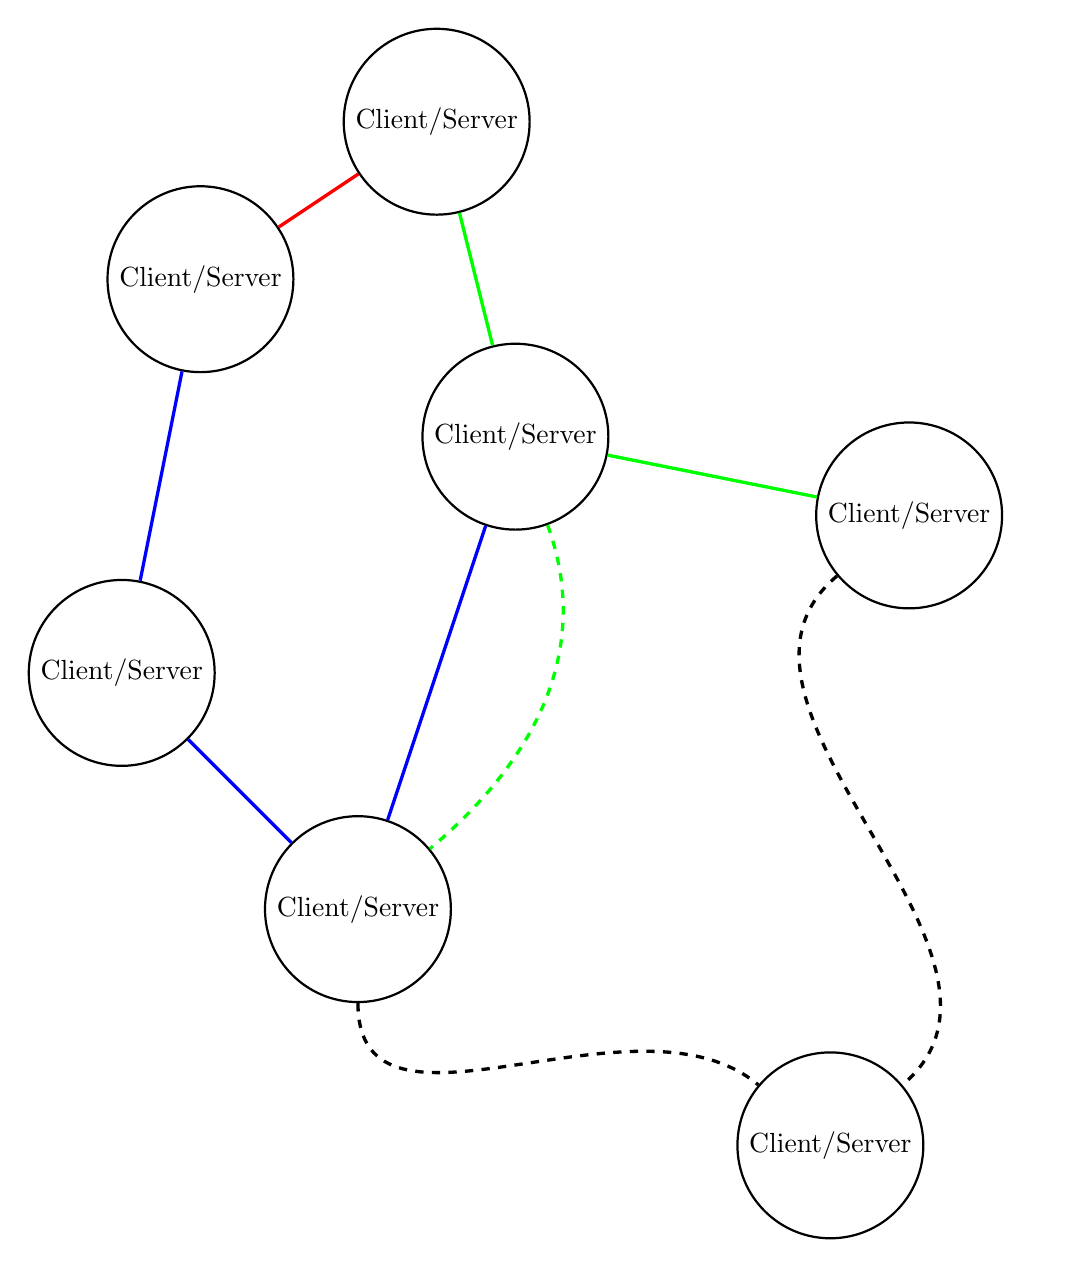
\begin{tikzpicture}
    \node[draw,circle] at (0,0) (1) {Client/Server};
    \node[draw,circle] at (3,-3) (2) {Client/Server};
    \node[draw,circle] at (5,3) (3) {Client/Server};
    \node[draw,circle] at (1,5) (4) {Client/Server};
    \node[draw,circle] at (10,2) (5) {Client/Server};
    \node[draw,circle] at (9,-6) (6) {Client/Server};
    \node[draw,circle] at (4,7) (7) {Client/Server};
    
    \draw[-, color=blue, very thick] (1) to (2);
    \draw[-, color=blue, very thick] (1) to (4);
    \draw[-, color=blue, very thick] (3) to (2);
    
    \draw[-, out=290, in=40, color=green, very thick, dashed] (3) to (2);
    \draw[-, color=green, very thick] (3) to (7);
    \draw[-, color=green, very thick] (3) to (5);
    
    \draw[-, out=220, in=40, very thick, dashed] (5) to (6);
    \draw[-, out=270, in=140, very thick, dashed] (2) to (6);
    
    \draw[-, color=red, very thick] (4) to (7);
  \end{tikzpicture}
  \caption[\textbf{Git-Netzwerkstruktur}]{Git-Netzwerkstruktur}
  \label{fig:Git}
  \label{figmin:Git}
\end{figure}

Für die Git-Verwaltung des Projekts wurde \iz{Github}{\url{https://github.com/}} verwendet. Um mit Github arbeiten zu können, wird ein gültiger Account vorrausgesetzt.
Mit Git kann in der Konsole gearbeitet werden oder es existieren Plugins für die IDE, was die Arbeit und Entwicklung weniger aufwendig macht.

An dieser Stelle soll kurz gezeigt werden, wie mit Git über die Konsole gearbeitet werden kann.

Ist bereits ein Git-Repositoty angelegt, kann wie folgt vorgegangen werden:

\begin{enumerate}
  \item das bereits existierende Verzeichnis mit dessen gesamten Inhalt wird 'geklont'. Danach können beliebige Veränderungen vorgenommen werden

	%% Listing: git clone
	\lstinputlisting[label={lst:git_clone},
	captionpos=b,
	belowcaptionskip=1pt,
	caption={Git: git clone},
	frame=tlbr, 
	language=java, 
	breaklines=true, 
	numbers=left,
	numberstyle=\tiny, 
	stepnumber=1, 
	numbersep=5pt, 
	basicstyle=\small\ttfamily,
	showstringspaces=true,
	keywordstyle=\bfseries\color{lila}, 
	backgroundcolor=\color{lightgrey}]{listings/git_clone.console}
	

  \item sollen die Änderungen wieder übernommen werden, müssen die entsprechenden Dateien hierfür übernommen werden. In diesem Fall werden durch den Parameter \texttt{*} alle Dateien im Verzeichnis hinzugefügt

	%% Listing: git add
	\lstinputlisting[
	label={lst:git_add},
	label={lstmin:git_add},
	captionpos=b,
	belowcaptionskip=2pt,
	caption={Git: git add},
	frame=tlbr, 
	language=java, 
	breaklines=true, 
	numbers=left, 
	numberstyle=\tiny, 
	stepnumber=1, 
	numbersep=5pt, 
	basicstyle=\small\ttfamily,
	showstringspaces=true,
	keywordstyle=\bfseries\color{lila}, 
	backgroundcolor=\color{lightgrey}]{listings/git_add.console}

  \item Anschließend müssen die Dateien für das Aktualisieren vorbereitet werden. Eine Nachricht ist hierzu notwendig und wird durch den Parameter \texttt{-m} angegeben

	%% Listing: git commit
	\lstinputlisting[label={lst:git_commit}, 
	captionpos=b,
	belowcaptionskip=2pt,
	caption={Git: git commit},
	frame=tlbr, 
	language=java, 
	breaklines=true, 
	numbers=left, 
	numberstyle=\tiny, 
	stepnumber=1, 
	numbersep=5pt, 
	basicstyle=\small\ttfamily,
	showstringspaces=true,
	keywordstyle=\bfseries\color{lila}, 
	backgroundcolor=\color{lightgrey}]{listings/git_commit.console}

  \item schließlich müssen wir die Dateien ans Repository übertragen. 

	%% Listing: git push
	\lstinputlisting[
	label={lst:git_push},
	label={lstmin:git_push},
	captionpos=b,
	belowcaptionskip=2pt,
	caption={Git: git push},
	frame=tlbr, 
	language=java, 
	breaklines=true, 
	numbers=left, 
	numberstyle=\tiny, 
	stepnumber=1, 
	numbersep=5pt, 
	basicstyle=\small\ttfamily,
	showstringspaces=true,
	keywordstyle=\bfseries\color{lila}, 
	backgroundcolor=\color{lightgrey}]{listings/git_push.console}

\end{enumerate}


Ist bisher noch kein Repository eingerichtet und ein neues soll erstellt werden, läuft der Vorgang wie folgt ab:

\begin{enumerate}

  \item Git initialisieren. In diesem Fall wird das aktuelle Verzeichnis also Git-Repository deklariert. In diesem kann später auch gearbeitet werden

	%% Listing: git init
	\lstinputlisting[label={lst:git_init}, 
	captionpos=b,
	belowcaptionskip=2pt,
	caption={Git: git init},
	frame=tlbr, 
	language=java, 
	breaklines=true, 
	numbers=left, 
	numberstyle=\tiny, 
	stepnumber=1, 
	numbersep=5pt, 
	basicstyle=\small\ttfamily,
	showstringspaces=true,
	keywordstyle=\bfseries\color{lila}, 
	backgroundcolor=\color{lightgrey}]{listings/git_init.console}

  \item Dateien die übertragen werden sollen, werden also dem Paket hinzugefügt (\texttt{add})
  
  \item die hinzugefügten Dateien werden für das Übertragen vorbereitet (\texttt{commit})
  
  \item nun muss ein Git-Repository (in diesem Fall auf Github) angelegt werden. In diesem Beispiel wird die Verbindung über \gls{HTTPS} aufgebaut. Git unterstützt aber ebenso auch Verbindungen über SSH. Diese sind generell aber mit etwas mehr Aufwand zu realisieren.   
  
  	%% Listing: git remote add
	\lstinputlisting[label={lst:git_remote_add}, 
	captionpos=b,
	belowcaptionskip=2pt,
	caption={Git: git remote add},
	frame=tlbr, 
	language=java, 
	breaklines=true, 
	numbers=left, 
	numberstyle=\tiny, 
	stepnumber=1, 
	numbersep=5pt, 
	basicstyle=\small\ttfamily,
	showstringspaces=true,
	keywordstyle=\bfseries\color{lila}, 
	backgroundcolor=\color{lightgrey}]{listings/git_remote_add.console}

  
  \item zuletzt können die vorgesehenen Daten dem Repository hinzugefügt (\texttt{push}) werden 
  
   
\end{enumerate}   
   
Allgemeine Informationen zu Git sind auf der \iz{Git-Website}{\url{http://git-scm.com/}} zu finden. Detailierte Hilfestellungen und die genaue Bedienungsanleitung kann in der offiziellen Git-Dokumentation \cite{GitDoku} nachgeschlagen werden. 
   
\subsubsection{JBoss Tools}
Ein weiteres praktisches Tool zur Entwicklungsunterstützung mit \ac{JSF} ist das JBoss-Tools Paket, welches über den Download im \iz{Eclipse-Marketplace}{\url{http://marketplace.eclipse.org/node/420896\#.UZS9yKwaSKI}} direkt bezogen werden kann.
Während der Programmierung einzelner Facelets rendert das Tools die dazugehörige Ansicht und stellt es dem Entwickler in Echtzeit dar. 

Das verschafft Vorteile beim Einstieg in Java Server Faces, aber auch dann, wenn bei der Implementierung schnell getestet werden soll.

\subsection{Java Server Faces}

JSF ist eine auf JAVA basierende Webtechnologie, die auf den Standards der Servlets- und JSP-Techniken aufsetzt.
Es ist ein eigenes plattformunabhängiges Framework zum vereinfachten Erstellen der Benutzeroberflächen in Webapps.
Dies wird dadurch erreicht, dass der Entwickler die Möglichkeit hat, die Benutzerschnittstellen auf eine einfache Art und Weise in eine Website einzubinden und die gesamte Navigation serverseitig zu definieren.
Darüber hinaus können alle clientseitigen Events an serverseitige Handler gebunden werden. 

Voraussetzungen zur Entwicklung mit JSF sind Grundkenntnisse mit der Programmiersprache JAVA und mit dem damit verbundenen \gls{JDK} sowie dem \gls{HTTP} Protokoll.
Zur Darstellung wird ein Servlet-Container, zum Beispiel ein Apache Tomcat, benötigt.
Für die Oberflächengestaltung der Webiste ist ein grundlegendes Verständnis der HTML-Technik von Vorteil.

Zunächst soll in diesem Abschnitt der Arbeit die grundlgende Funktionsweise des JSF-Standards dargestellt und beschrieben werden. 

\subsubsection{Das JSF-Prinzip}


Die zentrale Idee von JSF beruht auf dem Konzept der Komponenten. Diese fördern die Wiederverwendbarkeit des UI Codes in anderen Projekten und verhindern unnötige Coderverdopplung.


%% JSF Lifecycle
\begin{figure}[H]%[30]{r}{8cm}
\begin{center}
\scalebox{0.7}{
\begin{tikzpicture}[
  font=\sffamily,
  every matrix/.style={ampersand replacement=\&,column sep=2cm,row sep=2cm},
  source/.style={draw,thick,rounded corners,fill=yellow!20,inner sep=.3cm},
  process/.style={draw,thick,circle,fill=blue!20},
  sink/.style={source,fill=green!20},
  datastore/.style={draw,very thick,shape=datastore,inner sep=.3cm},
  dots/.style={gray,scale=2},
  to/.style={->,>=stealth',shorten >=1pt,semithick,font=\sffamily\footnotesize},
  every node/.style={align=center}]

  % Positionierung über Matrix-Layout
  \matrix{
     \node[process] (start) {Client};\&
      \node[source] (1st) {Restore View\\(Sicht wiederherstellen)}; \& \\
      \& \node[source] (2nd) {Apply Request Parameters\\ (Anforderungsparamter anwenden)}; \& \\
      \& \node[source] (3rd) {Process Validations\\ (Validierung ausführen)}; \& \\
      \& \node[source] (4th) {Update Model Values\\ (Modell aktualisieren)}; \& \\
      \& \node[source] (5th) {Invoke Application\\ (Anwendung ausführen)};\\
      
     \node[process] (end) {Client}; \&
      \node[source] (6th) {Render Response\\ (Antwort wiedergeben)}; \& \\
  };

  % VM - Host
  \draw[to, very thick] (start) -- node[midway,above] {Anforderung}
      node[midway,below] {} (1st);
  \draw[to, very thick] (1st) -- node[midway,above] {}
      node[midway,below] {} (2nd);
  \draw[to, very thick] (2nd) -- node[midway,above] {}
      node[midway,below] {} (3rd);
  \draw[to, very thick] (3rd) -- node[midway,above] {}
      node[midway,below] {} (4th);
  \draw[to, very thick] (4th) -- node[midway,above] {}
      node[midway,below] {} (5th);
  \draw[to, very thick] (5th) -- node[midway,above] {}
      node[midway,below] {} (6th);
  \draw[to, very thick] (6th) -- node[midway,above] {Antwort}
      node[midway,below] {} (end);
      
\end{tikzpicture}
}
\end{center}
\caption[\textbf{Diagramm des Lebenszyklus in JSF}]{Diagramm des Lebenszyklus in JSF}
\label{fig:IrianLfCycl}
\end{figure}

Um eine einheitliche Struktur der Anwendung zu schaffen, wird nach dem \ac{MVC} Prinzip das Modell, die Präsentation und die Steuerung voneinander getrennt, verdeutlicht wird dies unter \cite{IrianMVC}. Auch die \prettyref{fig:JSFMVC} erläutert das Modell im Bezug auf den JSF Lebenszyklus detailiert.

Unterstützt wird dieses Konzept durch die sogenannte View-Komponente, welche als Baumstruktur der JSF-Komponenten interpretiert werden kann. Jede JSF-Anwendung unterliegt einem Lebenszyklus, welcher auf der \prettyref{fig:IrianLfCycl} zu sehen ist, der View steht zu Beginn eines Zyklus.

%% Lebenszyklus
\begin{wrapfigure}[20]{r}{10cm}
\begin{center}
\scalebox{0.7}{
\begin{tikzpicture}[
  font=\sffamily,
  every matrix/.style={ampersand replacement=\&,column sep=2cm,row sep=2cm},
  source/.style={draw,thick,rounded corners,fill=yellow!20,inner sep=.3cm},
  process/.style={draw,thick,circle,fill=blue!20},
  sink/.style={source,fill=green!20},
  datastore/.style={draw,very thick,shape=datastore,inner sep=.3cm},
  dots/.style={gray,scale=2},
  to/.style={->,>=stealth',shorten >=1pt,semithick,font=\sffamily\footnotesize},
  every node/.style={align=center}]

  % Positionierung über Matrix-Layout
  \matrix{
     \node[process] (start) {Client};\&
      \node[source] (controller) {Servlet\\ (Controller)}; \& \\
      \& \& \\
      \& \& \node[source] (model) {JavaBean\\ (Model)}; \& \node[sink] (db) {Datenbank\\};\\
      \& \& \\
     \node[process] (end) {Client}; \&
      \node[source] (view) {Facelet\\ (View)}; \& \\
  };

  % Controller
  \draw[to, very thick] (start) -- node[midway,above] {1) Anfrage}
      node[midway,below] {} (controller);
  \draw[to, very thick] (controller) -- node[midway,right=0.2cm] {4) erzeugt/aktiviert}
      node[midway,below] {} (view);
  \draw[to, very thick] (controller) -- node[midway,right=1cm] {2) erzeugt/initialisiert}
      node[midway,below] {} (model);
      
  % Model
  \draw[to, very thick, dashed] (model) -- node[midway,above] {3) Daten}
      node[midway,below] {} (db);
  
  % View
  \draw[to, very thick] (view) -- node[midway,right=1cm] {5) bearbeitet}
      node[midway,below] {} (model);
  \draw[to, very thick] (view) -- node[midway,above] {6) Antwort}
      node[midway,below] {} (end);
      
\end{tikzpicture}
}
\end{center}
\caption[\textbf{Model-View-Controller Modell in JSF}]{Model-View-Controller Modell in JSF}
\label{fig:JSFMVC}
\end{wrapfigure}

Vor dem Ende des Zyklus wird das Wurzelelement des Views erneut rekursiv aufgerufen. Dieser Vorgang generiert die Antwort, welche bspw. eine HTML-Seite sein kann. Für die Deklaration der Web-ansicht
gibt es viele Möglichkeiten.
Die hier genannten Erklärungen zum Lebenszyklus einer JSF Anwendung sind in \cite{IrianLfCycl} beschrieben.
Betrachtet man bspw. andere Frameworks wie \gls{Turbine}, so dient als Seitendeklarationssprache, englisch \ac{VDL} genannt, \gls{Velocity} und bei \gls{Cocoon} ein abstrahierter XML-Dialekt. Bei JSF (und im übrigen auch bei \gls{Struts}) vor Version 2.0 wurden Java Server Pages eingesetzt.
Erst ab der Version 2.0 setzt JSF standardmäßig XHTML, bekannt als die sog. Facelets, auf welche in \prettyref{subsec:Darstellung von Seiteninhalten} näher eingegangen wird, als Seitendeklarationssprache ein. XHTML entwickelte sich aus HTML und XML, nachdem sich gezeigt hatte, dass HTML selbst nicht XML konform ist. XHTML wird als Schnittmenge aus HTML und XML verstanden (\cite{BaRiSch-WT}, 33).

Benutzereingaben können über eigene Komponenten oder mit einem Data Handler, aus JAVA Code bestehend, geschrieben werden. Diese Controller-Komponente entspricht dem Controller im \ac{MVC} Modell.
Die letzte Komponente, die Model-Komponente, beinhaltet die Logik der Webapp. In JSF sind diese Komponenten die sog. \gls{Java-Beans}, welche vom Servlet-Container verwaltet werden.

Die eigentliche Ansicht der Website, die dem Betrachter zur Verfügung gestellt wird, wird durch generierten HTML Code der Seite sichtbar, dies geschieht durch einen eigenen JSF-Renderer.
Darüber hinaus bietet JSF den Entwicklern weitere Möglichkeiten, sich eigene Renderer zusammenzustellen (\cite{WikiJSF01}).

\subsubsection{Darstellung von Seiteninhalten mit Facelets}\label{subsec:Darstellung von Seiteninhalten}
Bisher wurden lediglich Eindrücke, die auf die Konzeption und die allgemeine Verarbeitung von Informationen in JSF eingehen, vermittelt. Nun soll die Darstellung der Informationen durch JSF erklärt werden.

Die JSF-Technologie unterstützt, wie schon im vorherigen Abschnitt erwähnt, mehrere Arten zur Anzeige von Seiteninhalten. 
Vor Version JSF 2.0 wurde standardmäßig JSP als Seitendeklarationssprache eingesetzt, um die neu entwickelte Technologie zu etablieren und um für Entwickler die Probleme der Sprachbarrieren niedrig zu halten.
Da JSP noch immer ein weit verbreiteter Standard ist, wird es auch noch heute für JSF Projekte eingesetzt.
Das große Problem bei dieser Art der Implementierung ist, dass die Kombination von JSF und JSP keine gute Lösung darstellt. Die Problematik rührt daher, dass beide Technologien für unterschiedliche Einsatzzwecke entworfen wurden.

Wie oben schon beschrieben, wird eine JSF Applikation in mehreren Phasen abgearbeitet. Der Aufbau der Struktur von Komponenten und die Darstellung der Ausgabe wird hierbei in mehreren Phasen realisiert.
Im Gegensatz hierzu: JSP, welches mit nur einer einzigen Phase abgearbeitet wird. Die Antwort vom Server wird direkt in ihr ausgegeben. JSP Seiten stechen vor allem durch ihren Aufbau hervor.
Die Ausgabe, die der Sever darstellen muss, wird in einer JSP-Seite immer durch die Verwendung der JAVA-Funktion \texttt{out.println()} in HTML Seiten generiert, was zur Folge haben kann, dass Seiteninhalte vor anderen dargestellt werden oder das Design an Konsistenz verliert. Das geschieht vor allem dann, wenn normale HTML- und Text-Elemente zum Einsatz kommen.

Um diese Problematiken in den Griff zu bekommen, wurden die Facelets entwickelt. Hierbei handelt es sich ebenfalls um eine VDL, allerdings ist die dem Lebenszyklus von JSF-Applikationen angepasst.
Hierzu werden Inhalte aus XHTML-Dokumenten verknüpft um einen strukturierten Komponentenbaum aufzubauen.

%% Listing: eigene Komponente als Beispiel
	\lstinputlisting[label={lst:tree_form},
	caption={Hierarchische Struktur der einzelnen Facelet-Elemente},
	frame=tlbr, 
	language=java, 
	breaklines=true, 
	numbers=left, 
	numberstyle=\tiny, 
	stepnumber=1, 
	numbersep=5pt, 
	basicstyle=\small\ttfamily,
	showstringspaces=false,
	keywordstyle=\bfseries\color{lila}, 
	backgroundcolor=\color{lightgrey}]{listings/tree_form.xhtml}

Wie oben schon erwähnt, sind Facelets mittlerweile in JSF 2.0 zum Standard geworden, JSP wird nur noch aus Gründen der Kompatibilität unterstützt und besondere Features lassen sich in JSF sogar nur noch mit Hilfe von Facelets umsetzen. 

Aufgrund der Tatsache, dass Facelets speziell für JSF konzipiert und entwickelt wurden, bieten sie natürlich viele Vorteile.
Das Erstellen und Ausgeben von Seitenansichten wird mit Facelets effizienter. 
Dies schlägt sich in der Entwicklung von Seiten sowie in deren Geschwindigkeit beim Seitenaufbau nieder.

Zur Unterstützung der Wiederverwendbarkeit können JSF Seiten mit Hilfe der Facelets Template-basierend aufgebaut werden. Das bedeutet, dass komplette Seitenfragmente zentral abgelegt werden können und bei Bedarf in andere Seiten eingebettet werden. So kann bspw. ein Layout für einen Seitenkopf einmal definiert werden, um ihn dann später in anderen Seiten wiederverwenden zu können.
Dies verbessert zum einen die Wartbarkeit der Seiten und birgt den Vorteil der Modularisierung in ganzen Projekten.

Im Fall von \prettyref{lst:template}, welcher ein Beispiel des JSF-Templatings minimalistisch darstellt, wird ein HTML-Gerüst erzeugt. Es können zusätzlich globale CSS- und JavaScript-Dateien eingebunden werden.
Die Elemente \texttt{ui:insert} definieren Platzhalter für beliebige Daten, die an dieser Stelle eingefügt werden können.
Der \prettyref{lst:tree_form} zeigt eine Seite, die das gerade betrachtete Template verwendet.
Hierzu wurd im Element \texttt{ui:composition} das gewünschte Template zur Verwendung festgelegt. Nun wird mit \texttt{ui:define}, dessen \texttt{name}-Attribut dem \texttt{name}-Attribut des Elements \texttt{ui:insert} aus dem Template entsprechen muss, der Inhalt festgelegt.

%% Listing: eigene Komponente als Beispiel
	\lstinputlisting[
	label={lst:template},
	caption={Minimalbeispiel für ein Template},
	frame=tlbr, 
	language=java, 
	breaklines=true, 
	numbers=left, 
	numberstyle=\tiny, 
	stepnumber=1, 
	numbersep=5pt, 
	basicstyle=\small\ttfamily,
	showstringspaces=false,
	keywordstyle=\bfseries\color{lila}, 
	backgroundcolor=\color{lightgrey}]{listings/template.xhtml}
	
Wird der definierte \prettyref{lst:template} aufgerufen, so würde folgende HTML-Seite erzeugt werden:

%% Listing: eigene Komponente als Beispiel
	\lstinputlisting[label={lst:tree_form_rendered},
	caption={Gerenderte HTML-Seite des selbstdefinierten Templates},
	frame=tlbr, 
	language=java, 
	breaklines=true, 
	numbers=left, 
	numberstyle=\tiny, 
	stepnumber=1, 
	numbersep=5pt, 
	basicstyle=\small\ttfamily,
	showstringspaces=false,
	keywordstyle=\bfseries\color{lila}, 
	backgroundcolor=\color{lightgrey}]{listings/tree_form_rendered.xhtml}


Neben den Templates können auch komplett eigene Komponenten erstellt werden. Das ist vor allem dann vorteilhaft, wenn HTML-Code nach eigenen Vorstellungen eingebettet werden soll.
Hierzu wird über das \texttt{jsfc}-Attribut der Facelet-Compiler angewiesen, beliebige XML-Elemente in Komponenten umzuwandeln. 
Ein Beispiel zeigt der \prettyref{lst:custInputComponent}

	%% Listing: eigene Komponente als Beispiel
	\lstinputlisting[
	label={lst:custInputComponent},
	caption={Beispiel einer selbst erstellten Input-Komponente},
	frame=tlbr, 
	language=java, 
	breaklines=true, 
	numbers=left, 
	numberstyle=\tiny, 
	stepnumber=1, 
	numbersep=5pt, 
	basicstyle=\small\ttfamily,
	showstringspaces=true,
	keywordstyle=\bfseries\color{lila}, 
	backgroundcolor=\color{lightgrey}]{listings/custInputComponent.xhtml}
	
Im nächsten Abschnitt soll nun das dynamische Erzeugen von Seiten mit JSF erklärt werden.

\subsubsection{Managed-Beans in JSF}

In der Hierachie unter den Komponenten liegen die Managed-Beans (teilweise auch Backing-Beans genannt). Sie sind dafür verantwortlich, dass Werte zum 'Befüllen' von Komponenten geliefert werden. Diese Werte können Initialwerte sein, welche Managed Properties genannt werden.

Managed-Beans sind zentral definierte simple JAVA-Klassen, sogenannte \glspl{POJO}, die dem Java-Beans Standard entsprechen.
Je nach Gültigkeitsbereich, auch Scope genannt, der für die Managed-Beans deklariert ist, können diese für die gesamte Applikation oder nur für einzelne Benutzer gültig sein.
Deklariert werden können sie in der XML Konfiguration des JSF Projekts. Ab JSF 2.0 geht dies auch über Annotations über der Klassendefinition direkt im JAVA-Code. 

In JSF kann also auf die Eigenschaften der Managed-Beans, lesend und schreibend, zugegriffen werden. 
Eine solche Eigenschaft besteht aus einem Namen, einem Typ und \texttt{set}- und \texttt{get}-Methoden zum Lesen und Schreiben der Werte.
Die Namen solcher Methoden unterliegen gewissen Konventionen:
\begin{itemize}
  \item \texttt{get}[Eigenschaftsname]: lesender Zugriff
  \item \texttt{set}[Eigenschaftsname]: schreibender Zugriff
\end{itemize}

Der \prettyref{lst:UserBean.java} zeigt eine Managed-Bean Klasse mit jeweils 2 Methoden für einen der beiden privaten Strings der Klasse \texttt{firstName} und \texttt{lastName}.

	%% Listing: UserBean
	\lstinputlisting[
	label={lst:UserBean.java},
	caption={UserBean mit get- und set-Methoden},
	frame=tlbr, 
	language=java, 
	breaklines=true, 
	numbers=left, 
	numberstyle=\tiny, 
	stepnumber=1, 
	numbersep=5pt, 
	basicstyle=\small\ttfamily,
	showstringspaces=true,
	keywordstyle=\bfseries\color{lila}, 
	backgroundcolor=\color{lightgrey}]{listings/TestBean.java}

Dabei ist egal, ob mit den Methoden auf private Variablen zugegriffen wird oder ob komplexere Algorithmen ausgeführt werden, es ist in jedem Fall nur die Eigenschaft auf die zugegriffen wird, sichtbar.

Das dazugehörige Facelet stellt der \prettyref{lst:UserAdd1.xhtml} dar. Das Facelet zeigt ein kleines Eingabeformular, in welches einmal der Vorname und einmal der Nachname über Eingabefelder vom User eingegeben werden können. Im Facelet wird dies durch die Angabe der zu verwendenden Property \texttt{\#\{userBean.firstName\} } und \texttt{\#\{userBean.lastName\} } realisiert. Die Werte die im Textfeld eingegeben werden, werden auch von der Managed-Bean verarbeitet, indem die Setter-Methode, durch den Audruck des Attributs \texttt{value}, für das Feld \texttt{firstName} bzw. \texttt{lastName} der Bean \texttt{Customer} aufruft und die eingegebenen Werte weiter verarbeitet.

So kann also eine wichtige Aufgabe mit JSF relativ unproblematisch erledigt werden.
Nun sollen die Daten die ins Formular eingegeben werden weiterverarbeitet werden.
Hierzu wird im Formular der Button mit \texttt{action="sendUser()"} definiert. Beim Klick wird die Aktion \texttt{sendUser()} in der dazugehörigen Bean aufgerufen und die Daten aus dem Formular können wie gewünscht weiterverarbeitet werden.

Das gleiche Prinzip funktioniert ebenfalls für eine Ausgabe am Bildschirm, bspw. über den xhtml-Tag \texttt{h:outputText}. Es würde die relevante Getter-Methode aufgerufen werden und wiederum das dazugehörige Feld ausgegeben werden. 

	%% Listing
	\lstinputlisting[label={lst:UserAdd1.xhtml},
	caption={UserAdd Facelet zur UserBean mit Eingabeformular},
	frame=tlbr, language=XML, breaklines=true, 
	numbers=left, 
	numberstyle=\tiny, 
	stepnumber=1, 
	numbersep=5pt, 
	basicstyle=\small\ttfamily, 
	showstringspaces=true,
	keywordstyle=\bfseries\color{lila}, 
	backgroundcolor=\color{lightgrey}]{listings/TestFacelet_Eingabe.xhtml}

Ein Ausdruck beginnt immer mit den Zeichen \texttt{\$} oder \texttt{\#}. Begrenzt wird der Ausdruck durch geschweifte Klammern. Der Unterschied des \texttt{\$}-Zeichens zum \texttt{\#}-Zeichen ist, dass mit ihm nur lesend auf ein Property zugegriffen werden kann.
Der Ausdruck wird sofort evaluiert und ausgegeben. Er eignet sich daher für einfache Textausgaben.

Diese Ausdrücke sind Teil der \ac{UEL}, also eine Art von vordefinierten Facelet-Tags, mit deren Hilfe auf alle Properties einer Managed-Bean zugegriffen werden kann. 
	
	%% Listing
	\lstinputlisting[
	label={lst:UserAdd2.xhtml},
	label={lstmin:UserAdd2.xhtml},	
	caption={UserAdd Facelet zur UserBean mit Ausgabe},
	frame=tlbr, language=XML, breaklines=true, 
	numbers=left, 
	numberstyle=\tiny, 
	stepnumber=1, 
	numbersep=5pt, 
	basicstyle=\small\ttfamily, 
	showstringspaces=true,
	keywordstyle=\bfseries\color{lila}, 
	backgroundcolor=\color{lightgrey}]{listings/TestFacelet_Ausgabe.xhtml}

Die nachstehende Tabelle zeigt die möglichen Gültigkeitsbereiche für Managed-Beans:

% Scopes
\begin{table}[H]
\begin{center}
	\begin{tabular}{|l|l|l||}\hline
		\textbf{XML Wert} & \textbf{Annotation} & \textbf{Gültigkeitsbereich} \\ \hline	
		request & @RequestScoped & gültig solange der aktuelle Request behandelt wird\\ \hline \hline
		view & @ViewScoped & gültig solange die aktuelle View gültig ist\\ \hline \hline
		session & @SessionScoped & gültig für eine Session\\ \hline \hline
		application & @ApplicationScoped & gültig für die gesamte Applikation\\ \hline \hline
		none & @NoneScoped & gültig solange das Bean gültig ist\\ \hline \hline
	\end{tabular}
	\caption{Gültigkeitsbereiche für Managed-Beans}
	\label{tab:Scopes}
\end{center}
\end{table}

Der Tabelle kann entnommen werden, dass die verschiedenen Scopes auch unterschiedlich lange Lebensdauern in einer Webapplikation besitzen.
Spezialfall ist hier der Gültigkeitsbereich \texttt{@NoneScoped}. In diesem wird die Managed-Bean nicht gespeichert, sondern bei jedem Aufruf neu erstellt.
Der \texttt{@ApplicationScope}-Gültigkeitsbereich hingegen bildet den Gegensatz. Dieser gilt für die gesamte Lebendauer der App.

% Scope Lebendauern
\begin{wrapfigure}[13]{r}{10cm}
\centering\begin{tikzpicture}[decoration=penciline, decorate]
  
  % Repo
  \draw[very thick, ->] (0,0) -- (8,0) node[draw=white] at (5,-0.5) {Lebendauer $t$};
  
  % Application
  \draw (0,0.5) -- (0,1) -- (7,1) -- (7,0.5) -- (0,0.5) node[draw=white] at (0,1.5) {Application};
  \def \app{(0,0.5) -- (0,1) -- (7,1) -- (7,0.5) -- (0,0.5)}
  \fill[color=black, fill=green, fill opacity=0.8] \app;
  
  % Session
  \draw (0,2) -- (0,2.5) -- (5,2.5) -- (5,2) -- (0,2) node[draw=white] at (0,3) {Session};
  \def \sess{(0,2) -- (0,2.5) -- (5,2.5) -- (5,2) -- (0,2)}
  \fill[color=black, fill=green, fill opacity=0.8] \sess;
  
  % View
  \draw (0,3.5) -- (0,4) -- (3,4) -- (3,3.5) -- (0,3.5) node[draw=white] at (0,4.5) {View};
  \def \view{(0,3.5) -- (0,4) -- (3,4) -- (3,3.5) -- (0,3.5)}
  \fill[color=black, fill=green, fill opacity=0.8] \view;
  
  % Request
  \draw (0,5) -- (0,5.5) -- (1,5.5) -- (1,5) -- (0,5) node[draw=white] at (0,6) {Request};
  \def \re{(0,5) -- (0,5.5) -- (1,5.5) -- (1,5) -- (0,5)}
  \fill[color=black, fill=green, fill opacity=0.8] \re;
  
  
\end{tikzpicture}
\caption[\textbf{Scope Labensdauern}]{Scope Lebensdauern}
\label{fig:ScopeLfTme}
\end{wrapfigure}

\subsection{PostreSQL}

PostgreSQL ist quelloffen und ein sehr mächtiges objekt-relationales Datenbankmodell und -system. Mittlerweile unterliegt es mehr als 15 Jahren aktiver Entwicklung und wird stetig weiter verbessert. Aufgrund dieser langen Zeit konnte sich PostgreSQL einen guten Namen machen und wird aufgrund der Einfachheit, Daten zu integrieren und zu verwalten häufig eingesetzt.
Ein großer Vorteil von PostgreSQL ist desweiteren, dass es von allen gängigen Betriebssystemen wie Linux, Unix (BSD, Solaris, Mac OS X) und Windows unterstützt wird. Somit existieren auch grafische Benutzeroberflächen zur \ac{DB}-Verwaltung, wie das von uns eingesetzte \gls{pgAdmin III}.
Neben den Betriebssystemen werden auch nahezu alle gängigen Programmiersprachen unterstützt. Als Beispiele seien \gls{C/C++}, \gls{JAVA}, \gls{.Net}, \gls{Perl}, \gls{Python} und \gls{Ruby} genannt.
Diese allgemeinen Informationen, sowie die \prettyref{tab:PostgreSQLValues}, welche die Speicheverwaltungswerte auflistet, wurden der offiziellen PostgreSQL-Projektseite, welche unter \cite{PostgreSQLAllg} zu finden ist, entnommen. Ein Download-Paket des gesamten \ac{DB}-Systems kann unter \cite{PostgreSQLDwnld} bezogen werden. 

% Speicherverwaltung
\begin{table}[H]
\begin{center}
	\begin{tabular}{|l|l|}\hline
		\textbf{Limit} & \textbf{Wert} \\ \hline	
		Maximale DB Größe & Unbegrenzt \\ \hline \hline
		Maximale Tabellen Größe & 32 TB \\ \hline \hline
		Maximale Zeilen Größe & 1.6 TB \\ \hline \hline
		Maximale Feld Größe & 1 GB \\ \hline \hline	
		Maximale Anzahl der Zeile pro Tabelle & Unbegrenzt \\ \hline \hline
		Maximale Spalten pro Tabelle &	250 - 1600 abhängig vom Spaltentyp \\ \hline \hline
		Maximale Anzahl an Indizes per Tabelle & Unbegrenzt \\ \hline \hline
	\end{tabular}
	\caption{Speicherverwaltung von PostgreSQL}
	\label{tab:PostgreSQLValues}
\end{center}
\end{table}

Da das 'KuWaSys' mit JSF implementiert ist, ist eine \gls{JDBC}-Schnittstelle unter Zuhilfenahme eines PostgreSQL-Treibers zum Einsatz gekommen. Dieses Konzept bietet in Java die einfachste Möglichkeit auf eine PostgreSQL \ac{DB} zuzugreifen. Bei dem verwendeten Treiber handelt es sich um ein JDBC-Treiber des Typ-4. 
Typ-4 bedeutet, dass die JDBC-API Befehle direkt in \ac{DBMS} Befehle des jeweiligen Datenbankservers übersetzt werden.
Es wird kein Middleware-Treiber benötigt. 
Der Typ-4 ist damit der schnellste (wenn schnelle Netzwerkprotokolle verwendet werden) unter den vier verschiedenen Typen, dafür jedoch aufgrund der fehlenden Middleware weniger flexibel.
Dadurch ist ein Treiber des Typ-4 besonders gut für Webapps im Intranet geeignet, weshalb das 'KuWaSys' mit Hilfe des Typ-4 Treibers umgesetzt ist.

Der \prettyref{lst:JDBCCon} zeigt die Einbettung des JDBC-PostgreSQL Treibers in den JAVA Code. Dazu zeigt er einen beispielhaften Verbindungsaufbau zur Datenbank mit Default-Werten und eine Test-String Ausgabe. Das JDBC-PostreSQL \gls{JAR}-Paket wurde hierzu bereits in Eclipse integriert. Dies kann über den Einstellungs-Wizard in den Projekt-Eigenschaften bewerkstelligt werden. 

% Listing: JDBC SQL Connection
	\lstinputlisting[label={lst:JDBCCon},
	caption={Herstellung einer SQL-Konektivität in JAVA},
	frame=tlbr, language=java, breaklines=true, 
	numbers=left, 
	numberstyle=\tiny, 
	stepnumber=1, 
	numbersep=5pt, 
	basicstyle=\small\ttfamily, 
	showstringspaces=true,
	keywordstyle=\bfseries\color{lila}, 
	backgroundcolor=\color{lightgrey}]{listings/JDBCCon.java}